%% LaTeX Beamer presentation template (requires beamer package)
%% see http://bitbucket.org/rivanvx/beamer/wiki/Home
%% idea contributed by H. Turgut Uyar
%% template based on a template by Till Tantau
%% this template is still evolving - it might differ in future releases!

\documentclass{beamer}

\mode<presentation>
{  
\usetheme{Antibes}
\usecolortheme{seagull}

\setbeamercovered{transparent}
}



% font definitions, try \usepackage{ae} instead of the following
% three lines if you don't like this look
\usepackage{mathptmx}
\usepackage[scaled=.90]{helvet}
\usepackage{courier}
\usepackage[T1]{fontenc}

%%Pacotes
\usepackage[utf8]{inputenc} 
\usepackage[brazil]{babel} 


\title{OP-LSSVM}

%\subtitle{}

% - Use the \inst{?} command only if the authors have different
%   affiliation.
%\author{F.~Author\inst{1} \and S.~Another\inst{2}}
\author{David Clifte\inst{1}}

% - Use the \inst command only if there are several affiliations.
% - Keep it simple, no one is interested in your street address.
\institute[Universities of]
{

\inst{1}%
Department of Computer Science\\
Univ of S
}

\date{\today} % Data de hoje


% This is only inserted into the PDF information catalog. Can be left
% out.
\subject{Talks}



% If you have a file called "university-logo-filename.xxx", where xxx
% is a graphic format that can be processed by latex or pdflatex,
% resp., then you can add a logo as follows:

% \pgfdeclareimage[height=0.5cm]{university-logo}{university-logo-filename}
% \logo{\pgfuseimage{university-logo}}



% Delete this, if you do not want the table of contents to pop up at
% the beginning of each subsection:
\AtBeginSubsection[]
{
	\begin{frame}<beamer>
	\frametitle{Outline}
	\tableofcontents[currentsection,currentsubsection]
	\end{frame}
}

% If you wish to uncover everything in a step-wise fashion, uncomment
% the following command:

%\beamerdefaultoverlayspecification{<+->}

\begin{document}

	\begin{frame}
	\titlepage
	\end{frame}

\begin{frame}
	\frametitle{Outline}
	\tableofcontents
	% You might wish to add the option [pausesections]
\end{frame}


\section{Regression Shirinkage and SubsetSelection}

\subsection{Least Squares Regression}
\begin{frame}
	The method of least squares is a standard approach in regression analysis to the
	approximate solution of overdetermined systems, i.e., sets of equations in which
	there are more equations than unknowns. "Least squares" means that the overall
	solution minimizes the sum of the squares of the errors made in the results of
	every single equation.

\begin{figure}[h!] \caption{Mínimos Quadráticos.} \centering
	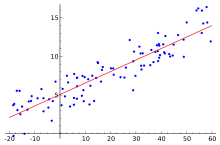
\includegraphics[width=0.5\textwidth]{imagens/lsr.png} 
\end{figure}
\end{frame}
 



\begin{frame}
	\begin{equation}
		y = \alpha + \beta x + \varepsilon
	\end{equation}
	
	\begin{itemize}{}
	\item  $\alpha$ : Parâmetro do modelo chamado de constante (porque não depende
	de x).
	\item $\beta$ : Parâmetro do modelo chamado de coeficiente da variável x.
	\item   $\varepsilon$ : Erro - representa a variação de y\,\! que não é
	explicada pelo modelo.
	\end{itemize}
	
	Minimizar:
	\begin{align}
	\sum_{i=1}^n e_i^2
	\end{align}

\end{frame}


\begin{frame}
	\begin{align}
	\sum_{i=1}^n e_i^2
	\\
	e_i = y_i - a - b x_i
	\\
	S(a,b) = \sum_{i=1}^n \left( y_i - a - b x_i \right) ^2
	\\
	\frac{\partial S}{\partial a}  = -2 \sum_{i=1}^n ( y_i - a - b x_i ) = 0 
	\\
	\frac{\partial S}{\partial b}  = -2 \sum_{i=1}^n x_i  ( y_i - a - b x_i  ) = 0 \\
	\end{align}
	
	\begin{figure}
	  \centering
	  \subfloat  {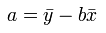
\includegraphics[width=3cm]{imagens/e1.png}}\qquad
	  \subfloat  {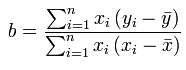
\includegraphics[width=3cm]{imagens/e2.png}}
	\end{figure}
\end{frame}  


\subsection{LASSO}

\begin{frame}
Semelhante aos mínimos quadráticos porém é inserida mais uma restrição além da
minimização do erro quadrárico.
Com a limitação do somatório dos coeficientes angulares temos que estes mesmos
coeficientes tenderão a valores próximos de zero e portanto alguns deles poderão
ser removidos.

\begin{align}
	\sum_{i=1}^n e_i^2
	\\
	e_i = y_i - a - b x_i
	\\
	\sum_{j=1}^n abs(b_j) < c
\end{align}
\end{frame}


\subsubsection{Forward selection}

\begin{frame}
\textbf{ Forward selection}: which involves starting with no variables in the
model, testing the addition of each variable using a chosen model comparison criterion,
adding the variable (if any) that improves the model the most, and repeating
this process until none improves the model.

\begin{itemize}
\item Start with all coefficients bj equal to zero.
\item Find the predictor xj most correlated with y, and add it into the model.
Take residuals r= y-yhat.
\item Continue, at each stage adding to the model the predictor most correlated
with r.
\item Until: all predictors are in the model
\end{itemize}

\end{frame}

\subsubsection{LARS}


\begin{frame}
\textbf{ Least angle regression algorithm:}
	\begin{itemize}
	\item Start with all coefficients bj equal to zero.
	\item Find the predictor xj most correlated with y
	\item Increase the coefficient bj in the direction of the sign of its
	correlation with y. Take residuals r=y-yhat along the way. Stop when some other predictor xk has as much correlation with r as xj has.
	\item Increase (bj, bk) in their joint least squares direction, until some other
	predictor xm has as much correlation with the residual r.
	\item Continue until: all predictors are in the model
	\end{itemize}
\end{frame}


\section{OP-ELM}

\subsection{ELM}

\begin{frame}
Foi desenvolvido para redes com apenas
duas camadas: a camada de entrada e a
camada escondida;

Os pesos de entrada $W$ e os bias da camada
escondida são escolhidos aleatoriamente;

Os pesos da camada de saída, $\beta$ são
determinados analiticamente (i. e., não há
ciclos iterativos para ajuste de parâmetros).


\end{frame}

\begin{frame}
	Considere um conjunto de M amostras distintas $(x_i,y_i)$ onde $x_i \in
	\Re^{d_1}$ e $y_i \in \Re^{d_2}$.
	
	A saída do ELM para um dado $x_j$ pode ser computada assim:
	
	\begin{equation}
	y_j= \sum_{i=1}^{N} \beta_i f(w_i x_j + b_i)
	\end{equation}
	
	Simplificando na forma de vetores temos:
	\begin{align}
		X_j = \begin{bmatrix}
					 1 & x_1 & x_2 & ...& x_m
			  \end{bmatrix} \\
% 		W=w_{ij} = \begin{bmatrix}
% 					 w_{11} &  w_{1j} & w_{1N} \\
% 					 w_{i1} &  w_{ij} & w_{iN} \\
% 					 w_{M1} &  w_{Mj} & w_{MN} \\
% 			  \end{bmatrix}\\
		H = f(X_j W)\\
		H \beta  = Y \\
		\beta = H^{\dagger} Y
	\end{align}
\end{frame}


\begin{frame}
	\frametitle{}
	\framesubtitle{Subtitles are optional}
	
	\begin{itemize}
	  \item
	  \item
	\end{itemize}
\end{frame}



\section{OP-LSSVM}


\section*{Summary}

\begin{frame}
\frametitle<presentation>{Summary}

\begin{itemize}
  \item The \alert{first main message} of your talk in one or two lines.
\end{itemize}

% The following outlook is optional.
\vskip0pt plus.5fill
\begin{itemize}
  \item Outlook
  \begin{itemize}
    \item Something you haven't solved.
    \item Something else you haven't solved.
  \end{itemize}
\end{itemize}
\end{frame}

\end{document}
